\section{Introduction}

We address the task of determining whether a string belongs to a specified language. 
Automata serve as abstract machines employed to apply a procedure for string recognition.
In this context, the input domain consists of a set of strings from an alphabet $\Sigma$.
The application of a recognition algorithm $\alpha$ to a given string $x$ is expressed as $\alpha(x)$.
\begin{definition}[\textit{Accepted string}]
    A string $x$ is deemed accepted if $\alpha(x) = \textnormal{yes}$; otherwise, it is rejected.
\end{definition}
\begin{definition}[\textit{Recognized language}]
    The language recognized, $L(\alpha)$, is the set of accepted strings:
    \[L(\alpha)=\{x \in \Sigma^{\ast}\mid \alpha(x)=\textnormal{yes}\}\]
\end{definition}
In cases where the language is semidecidable, there is a possibility that the algorithm may not terminate for some incorrect string $x$.
However, in the practical realm of language processing, concerns about decidability issues are alleviated, as the relevant language families are typically decidable.
\begin{definition}[\textit{Computation step}]
    In both theoretical and practical considerations of formal languages, a computation step is defined as a singular atomic operation of the automaton, capable of manipulating only one symbol at a time. 
\end{definition}
Consequently, it is customary to articulate the recognition algorithm through an automaton, be it a recognizer or a transducer machine. 
This convention serves two primary purposes:
\begin{enumerate}
    \item Establishing a clear connection between different language families and their respective generative devices.
    \item Deferring unnecessary and premature references to the concrete implementation of the algorithm in a specific programming language.
\end{enumerate}
\begin{figure}[H]
    \centering
    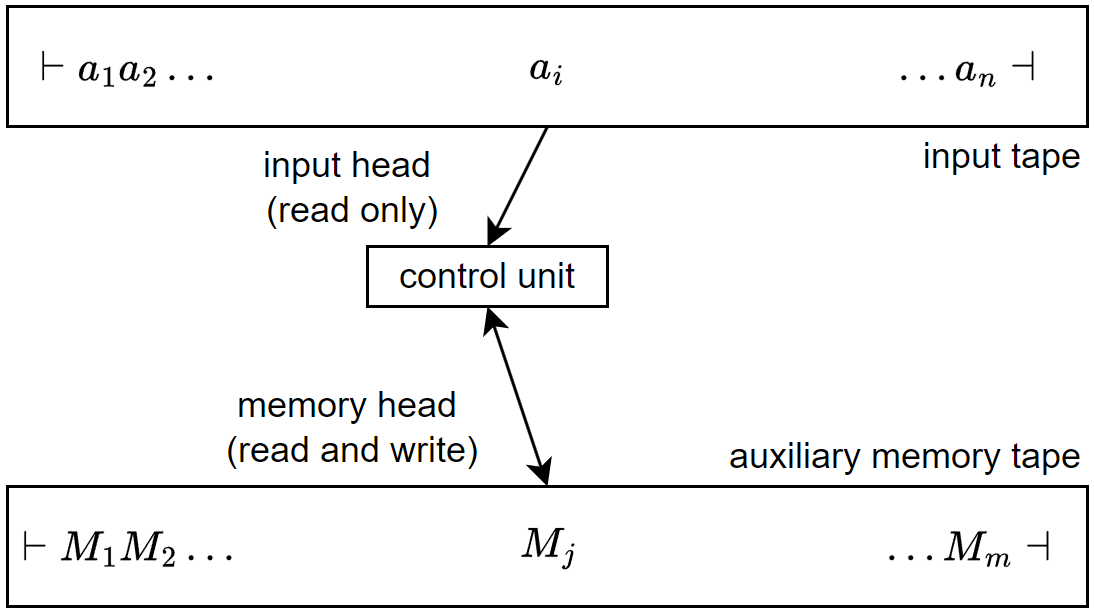
\includegraphics[width=0.5\linewidth]{images/fsa.png}
    \caption{General model of a recognizer automaton}
\end{figure}

\paragraph*{Moves}
The automata scrutinize the input string and carry out a sequence of moves, with each move contingent upon the symbols currently indicated by the heads and the ongoing state. 
These moves may have various effects, including:
\begin{itemize}
    \item Shifting the input head one position to the left or right.
    \item Replacing the current memory symbol with a new one and shifting the memory head one position to the left or right.
    \item Changing the current state.
\end{itemize}
Depending on the type of automaton, certain characteristics can emerge:
\begin{itemize}
    \item \textit{One-way automaton}: the input head is capable of shifting only to the right.
    \item \textit{No auxiliary memory}: represented by finite state automata, this machine model recognizes regular languages.
    \item \textit{Auxiliary memory}: illustrated by pushdown automata, this machine model recognizes free languages.
\end{itemize}
\begin{definition}[\textit{Automaton configuration}]
    A configuration comprises three components determining the automaton's behavior: the unread segment of the input tape, the contents and position of the memory tape and head, and the current state of the control unit.
\end{definition}
In the initial configuration, the input head is positioned on the symbol immediately following the start-marker, the control unit is in a specific state (initial state), and the memory tape contains only a special initial symbol.
Transitions, driven by moves, prompt changes in the automaton configuration. 
The entire sequence of transitions constitutes the computation of the automaton.
\begin{definition}[\textit{Deterministic automaton}]
    An automaton displays deterministic behavior if, in every instantaneous configuration, at most one move is possible. 
    Otherwise, the automaton is termed non-deterministic.
\end{definition}
In the final configuration, the control unit occupies a designated final state, and the input head is positioned on the end-marker of the string to be recognized. 
Sometimes, the final configuration is characterized by a condition for the memory tape: either empty or containing only one special final symbol.

\begin{definition}[\textit{Acceptance condition}]
    A source string $x$ is accepted by the automaton when it initiates from the initial input configuration $\vdash x \dashv$, undergoes a series of transitions, and arrives at a final configuration.
\end{definition}
The collection of all strings accepted by the automaton forms the language recognized by it.
In the case of non-deterministic automata, it might achieve the same final configuration through different sequences of transitions, or it could even reach multiple distinct final configurations.
he computation concludes either when the automaton reaches a final configuration or when it cannot perform any further transition steps because there are no possible moves left in the current instantaneous configuration. 
In the former scenario, the input string is accepted; in the latter, it is rejected.
\begin{definition}[\textit{Equivalence}]
    Two automata that recognize the same language are termed equivalent.
\end{definition}
Regular languages, recognized by finite state automata, constitute a subset of languages recognizable in real time by a Turing machine.
Conversely, context-free languages form a subset of languages recognized by a Turing machine with polynomial time complexity.
Numerous applications in computer science and engineering leverage finite state automata, including digital design, control theory, communication protocols, the exploration of system reliability and security, and more.